\chapter{Results}\label{chap:results}
This chapter outlines the fit results from the functional fit to the data and corresponding profile likelihood fit to the data. The statistical analysis is also presented where results are presented in the context of model independent and model dependent CI signals. 

\section{Fits to data}
The background only fits and extrapolation to the data in the signal regions considered in the analysis are shown in \cref{fig:fits}. The fits are performed in the \SI{1}{\giga\electronvolt} linear binned datasets corresponding to the full Run-2 luminosity of \SI{139}{\femto\barn^{-1}}. The CR choices corresponding the the SR choice is defined in \cref{sec:extrap:optimisation}. The linear binning is used as it allows for a better constrained fit to the data in the CR. However, the linear binning is less appealing to present the fits as it becomes difficult to determine any features in the distribution due to the large number of bins. The parameter values from the fit to the data in the CR is given in \cref{tab:fitpars}. 

\cref{fig:fits} depicts the extrapolation to the SR, where the contents of the SR has been integrated into a single bin to be consistent with the statistical analysis. The uncertainty on the background estimate in the SR as well as some benchmark CI models are also depicted in the figure. The bottom panel outlines the pulls for each data point, defined as $(\mathrm{Data}-\mathrm{Fit})/\sigma\mathrm{Data}$. The distribution are presented in $\log{(\text{m}_{\ell\ell})}$ to allow for a cleaner presentation of the fits. 

\begin{figure}[!htpb]
    \centering
    \begin{subfigure}[b]{0.49\textwidth}
        \centering
        \includegraphics[width=\textwidth]{/Users/Deshan/Documents/PhD/thesis/Thesis/figures/results/fig_02a.pdf}
        \label{fig:fits1}
    \end{subfigure}
    \begin{subfigure}[b]{0.49\textwidth}
        \centering
        \includegraphics[width=\textwidth]{/Users/Deshan/Documents/PhD/thesis/Thesis/figures/results/fig_02b.pdf}
        \label{fig:fits2}
    \end{subfigure}
    \begin{subfigure}[b]{0.49\textwidth}
        \centering
        \includegraphics[width=\textwidth]{/Users/Deshan/Documents/PhD/thesis/Thesis/figures/results/fig_02c.pdf}
        \label{fig:fits3}
    \end{subfigure}
    \begin{subfigure}[b]{0.49\textwidth}
        \centering
        \includegraphics[width=\textwidth]{/Users/Deshan/Documents/PhD/thesis/Thesis/figures/results/fig_02d.pdf}
        \label{fig:fits4}
    \end{subfigure}
    \caption[Distributions of the invariant mass of dilepton pairs passing the full selection for dielectrons and dimuons. Where the background-only fit has been performed in the CR and extrapolated to the signal region.]{
    Distributions of the invariant mass of dilepton pairs passing the full selection for dielectrons (left) and dimuons (right), and showing CR and SR for constructive interference (top) and destructive interference (bottom).
    The data points are plotted at the centre of each bin as the number of events divided by the bin width, which is constant in $\log{(\text{m}_{\ell\ell})}$.
    The error bars indicate statistical uncertainties only.
    A few CI benchmark signal shapes are shown, scaled to the data luminosity and superimposed by subtracting the LO DY component and adding the resulting shape to the background shape obtained from the fit.
    These signals have LL chirality with $\Lambda=$ 18, 22, and 26~TeV for the constructive case and $\Lambda=$16, 20, and $26$~TeV for the destructive case.
    The background-only fit is shown in solid red, with the light red area being its uncertainty.
    The boundaries of the CR and SR corresponding to the signals used are shown in dotted vertical lines for reference and marked by arrows.
    %In the destructive interference case, the signal shapes do not differ much on the scale used for these plots.
    The differences between the data and the fit results in units of standard deviations of the statistical uncertainty are shown in the bottom panels.
    }
    \label{fig:fits}
\end{figure}

\begin{table}[htp]
    \centering
    {\footnotesize
    \begin{tabular}{l | c c | c c}
    \toprule
    Parameter  &  \ee, Constructive &  \ee, Destructive &  $\mumu$, Constructive &  $\mumu$, Destructive \\
    \hline
    a & $(6.17\times \pm 0.02)\times 10^{-3}$ & $7.87\pm 0.03)\times 10^{-3}$ & $(6.90\pm 0.03)\times 10^{-6}$ & $(4.39\pm 0.02)\times 10^{-7}$ \\
    b (fixed) & 6.1 & 6.1 & 1.3 & 1.3 \\
    c (fixed) & 1/2 & 1/2 & 1/3 & 1/3 \\
    $p_0$ & -12.3$\pm$0.1 & -12.2$\pm$0.1 & -14.9$\pm$0.2 & -17.0$\pm$0.2 \\
    $p_1$ & -4.15$\pm$0.02 & -4.16$\pm$0.03 & -4.41$\pm$0.04 & -4.70$\pm$0.04 \\
    $p_2$ & -0.944$\pm$0.005 & -0.945$\pm$0.006 & -0.927$\pm$0.008 & -0.846$\pm$0.008\\
    $p_3$ & -0.0832$\pm$0.0008 & -0.083$\pm$0.001 & -0.081$\pm$0.001 & -0.064$\pm$0.001\\
    \bottomrule
    \end{tabular}
    }
    \caption[Parameters for the functional form given in Eq.~\cref{eq:fitfunc} in each of the signal regions considered in the analysis.]{Parameters for the functional form given in Eq.~\cref{eq:fitfunc} in each of the signal regions considered in the analysis. The uncertainties are statistical only.}
    \label{tab:fitpars}
\end{table}

ATLAS Event displays for the highest mass dielectron and dimuon candidates are shown in \cref{fig:eventDisplay}. The dielectron candidate with the highest mass reconstructed mass corresponds to an electron pair with $m_{ee} = \SI{4.06}{\tera\electronvolt}$. The electrons are emitted back to back with a leading electron $\et = \SI{2.01}{\tera\electronvolt}$, $\eta = 0.47$ and $\phi = -0.78$. Whereas, the subleading electron is emitted with $\et = \SI{1.92}{\tera\electronvolt}$, $\eta = 0.03$ and $\phi = 2.37$. The dimuon highest mass candidate has $m_{\mu\mu} = \SI{2.75}{\tera\electronvolt}$. The leading muon is emitted with $\pt = \SI{1.82}{\tera\electronvolt}$, $\eta = -0.52$ and $\phi = -0.56$, and the subleading muon has $\pt = \SI{1.04}{\tera\electronvolt}$, $\eta = -0.67$ and $\phi = 2.53$. Figure \cref{fig:eventDisplay} depicts jets overlapping with the muons, where the \pt < \SI{50}{\giga\electronvolt}, therefore, indicating that they are induced by the calorimeter deposits of the muons. 



\subsubsection{Signal region Yields and significances}

\cref{tab:yields} lists the expected background and observed event yields in each of the SR defined in \cref{sec:extrap:optimisation}. The background uncertainties are also shown in terms of numbers of events in the signal region. A single bin Poisson likelihood is constructed for each of the SR as described in \cref{chap:stats} and the compatibility of finding the observed data with the background-only hypothesis is tested by fitting the data with the statistical model. The largest deviation from the expected background can be seen in the electron constructive signal region, which corresponds to a observed significance of $1.4\sigma$. There is a small deficit of events observed in the other SRs, where the observed significances range from $0.16\sigma$ to $0.61\sigma$. The significances were calculated using the profile likelihood test statistic and 500000 MC toy experiments. The results indicate that there are no significant excesses observed in the data in the SRs to hint at the presence of new physics signatures. 

\begin{figure}[!htpb]
    \centering
    \begin{subfigure}[b]{0.49\textwidth}
        \centering
        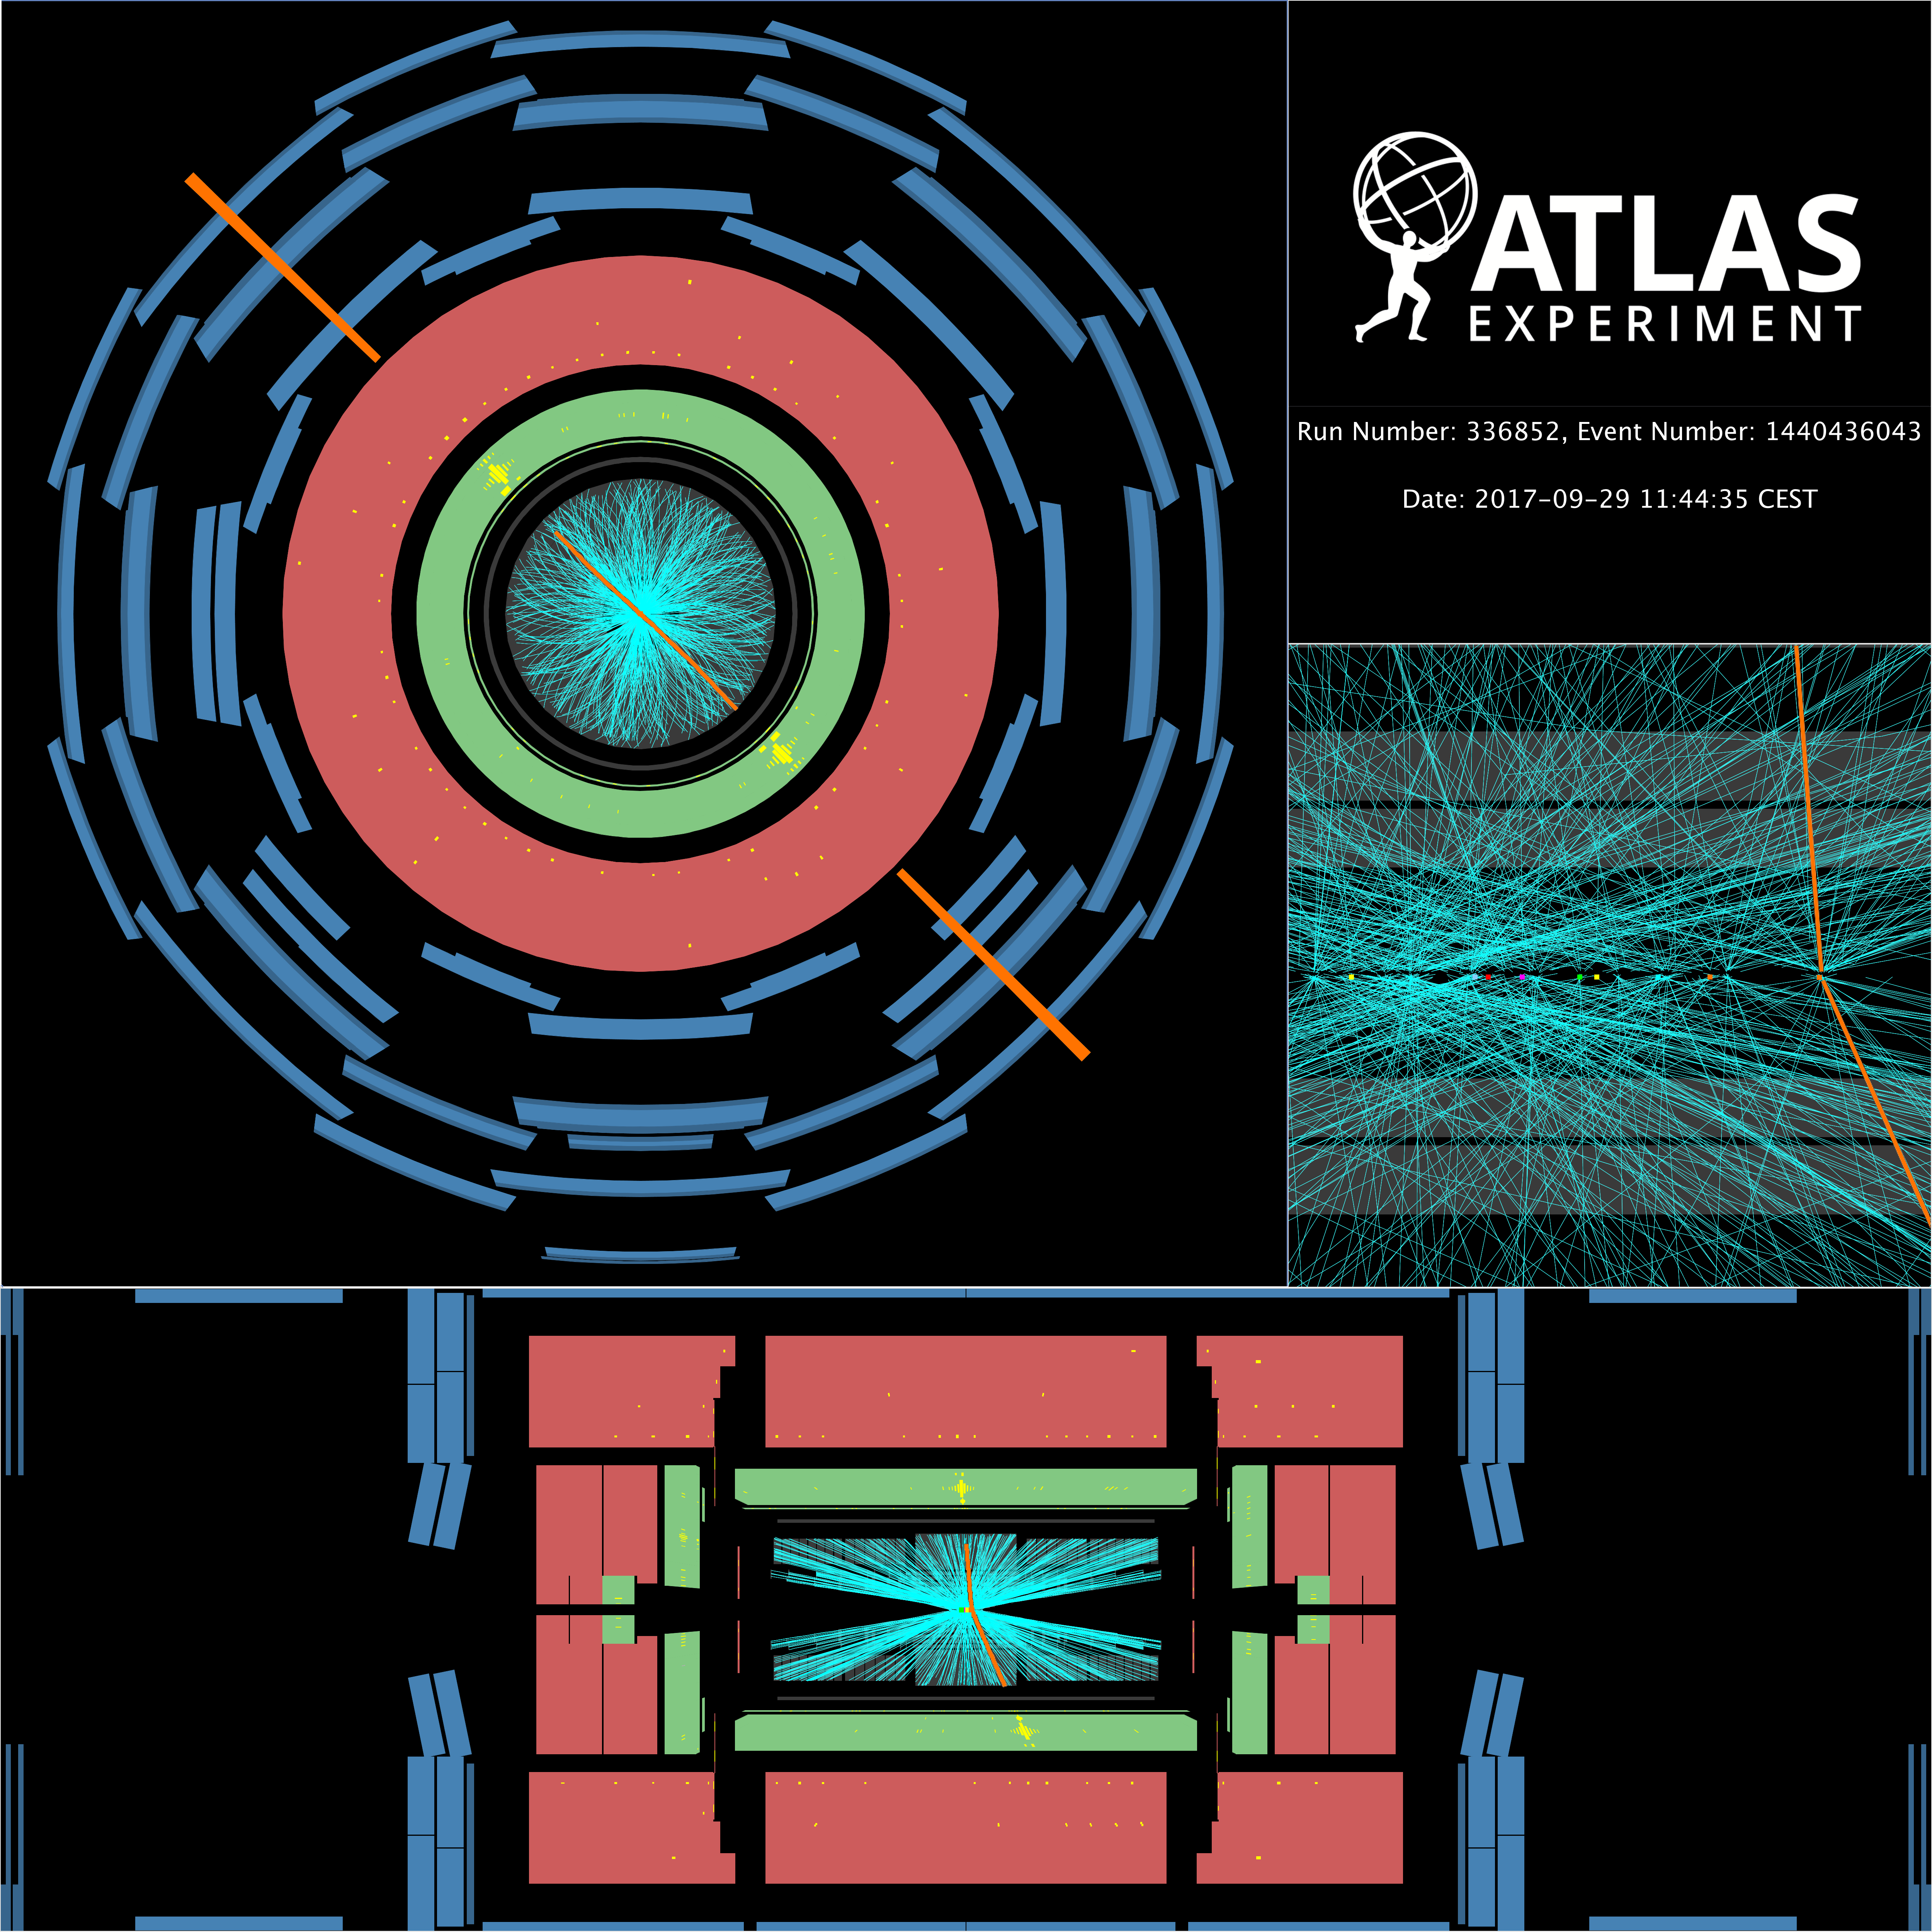
\includegraphics[width=\textwidth]{/Users/Deshan/Documents/PhD/thesis/Thesis/figures/results/electron_eventDisplay.png}
        \label{fig:eventDisplay1}
    \end{subfigure}
    \begin{subfigure}[b]{0.49\textwidth}
        \centering
        \includegraphics[width=\textwidth]{/Users/Deshan/Documents/PhD/thesis/Thesis/figures/results/muon_eventDisplay.png}
        \label{fig:eventDisplay2}
    \end{subfigure}
    \caption[Event display of the dielectron and dimuon candidate with the highest invariant mass in the 2015--2018 data taking period]{
    Event display of the dielectron (left) and dimuon (right) candidate with the highest invariant mass in the 2015--2018 data taking period with $m_{\mu\mu}$ = \SI{2.75}{\tera\electronvolt} and $m_{ee}$ = \SI{4.06}{\tera\electronvolt}~\cite{Aad:2019fac}.
    }
    \label{fig:eventDisplay}
\end{figure}

\begin{table}[htp]
\begin{center}
\begingroup
\setlength{\tabcolsep}{9pt} % Default value: 6pt
\renewcommand{\arraystretch}{1.5} % Default value: 1
{\small
\begin{tabular}{l l | c c | c c c c | c }
\toprule
\multicolumn{2}{c|}{Signal Regions} & \multicolumn{2}{c|}{Yields} & \multicolumn{4}{c|}{Background Uncertainties} & Significance \\
Channel & Interference & Data & Background & \STATU & \ISSU & \CRBU & Total & \\
\hline
\ee     & Constructive & 19 & 12.4 & 1.7 & 0.5 & 0.2 & 1.8 & 1.44$\sigma$\\
\ee     & Destructive  & 2  & 3.1  & 1.1 & 0.2 & <0.1 & 1.1 & 0.19$\sigma$\\
$\mumu$ & Constructive & 6  & 9.6  & 2.0 & 0.6 & 0.2 & 2.1 & 0.61$\sigma$\\
$\mumu$ & Destructive  & 1  & 1.4  & 0.8 & 0.3 & 0.1 & 0.9 & 0.17$\sigma$\\
\bottomrule
\end{tabular}
}
\endgroup
\caption[The dielectron and dimuon event yields for the data, the expected background, the corresponding background uncertainties and the respective significances in the different signal regions used in the analysis.]{The dielectron and dimuon event yields for the data, the expected background, the corresponding background uncertainties and the respective significances in the different signal regions used in the analysis. \STATU is the ``statistical uncertainty'', \ISSU is the ``induced spurious signal uncertainty'' and \CRBU is the ``control region bias uncertainty''. The total uncertainty is calculated by taking the sum in quadrature of the individual components. The significance of an excess is quantified by the probability (p-value) of the observed data given the background-only hypothesis}
\label{tab:yields}
\end{center}
\end{table}

\section{Nuisance parameter rankings}

The pulls and impact of the nuisance parameters are checked in order to determine if their values have significantly from the original estimate after the fit. The procedure outlined in \cref{sec:stats:nps} is used to calculate the pulls and impact of the nuisance parameters. The pulls and impact are estimated using the model independent description of the statistical model, where $\nu_s$ is taken as the POI. They and are presented in \cref{fig:nprankingee,fig:nprankingmm} for the electron and muon channels, respectively, in the SRs considered in the analysis. Only the uncertainties on the background estimate and the luminosity uncertainty on the signal event yield are considered in the model independent description, due to there being no explicitly defined signal model. 

The nuisance parameters are ranked based on their \emph{postfit} impact, where the nuisance parameters are shown according to their impact in descending order. The dominant uncertainty in all signal regions and channels considered is the statistical uncertainty of the fit (\STATU), indicating that the sensitivity to non-resonant signals is statistically dominated. The second largest impact is from the induced spurious signal uncertainty (\ISSU). The contribution from the luminosity ($\sigma_{Lumi})$ and \CRBU have a negligible impact on the results. The pulls indicate that there are no visible pulls on the nuisance parameters and that they are not constrained, which can be determined by the error bar on the pull. An error on the pull smaller or larger than $1\sigma$ would indicate that a nuisance parameter has been constrained \emph{postfit}. Differences between the \emph{postfit} and \emph{prefit} impacts can be inferred from the error bar on the pull, as any residual difference would indicate that the nuisance parameter is constrained. 


\begin{figure}[!htpb]
    \centering
    \begin{subfigure}[b]{0.49\textwidth}
        \centering
        \includegraphics[width=\textwidth]{/Users/Deshan/Documents/PhD/thesis/Thesis/figures/results/plot_NPranking_nSig_ee_const_workspace_top4.pdf}
        \label{fig:npranking1}
    \end{subfigure}
    \begin{subfigure}[b]{0.49\textwidth}
        \centering
        \includegraphics[width=\textwidth]{/Users/Deshan/Documents/PhD/thesis/Thesis/figures/results/plot_NPranking_nSig_ee_dest_workspace_top4.pdf}
        \label{fig:npranking2}
    \end{subfigure}
    \caption[Ranking plots for the considered systematic uncertainties for the model independent limits in the electron channel signal regions]{Ranking plots for the considered systematic uncertainties for the model independent limits. The impact on the parameter of interest ($\nu_s$) is shown in the signal regions considered in the electron channel. The systematic uncertainties are listed in decreasing order of impact on the parameter of interest. The red and blue bards correspond to the postfit upward and downward variations, respectively, where the impact is referred to on the upper axis. The pulls of the corresponding nuisance parameters are shown by the marked circle, where the pulls are referred to in the bottom axis. The constraint of the nuisance parameter is indicated by the black error bar. 
    }
    \label{fig:nprankingee}
\end{figure}

\begin{figure}[!htpb]
    \centering
    \begin{subfigure}[b]{0.49\textwidth}
        \centering
        \includegraphics[width=\textwidth]{/Users/Deshan/Documents/PhD/thesis/Thesis/figures/results/plot_NPranking_nSig_mm_const_workspace_top4.pdf}
        \label{fig:nprankin3}
    \end{subfigure}
    \begin{subfigure}[b]{0.49\textwidth}
        \centering
        \includegraphics[width=\textwidth]{/Users/Deshan/Documents/PhD/thesis/Thesis/figures/results/plot_NPranking_nSig_mm_dest_workspace_top4.pdf}
        \label{fig:nprankin4}
    \end{subfigure}
    \caption[Ranking plots for the considered systematic uncertainties for the model independent limits in the muon channel signal regions]{Ranking plots for the considered systematic uncertainties for the model independent limits. The impact on the parameter of interest ($\nu_s$) is shown in the signal regions considered in the muon channel. The systematic uncertainties are listed in decreasing order of impact on the parameter of interest. The red and blue bards correspond to the postfit upward and downward variations, respectively, where the impact is referred to on the upper axis. The pulls of the corresponding nuisance parameters are shown by the marked circle, where the pulls are referred to in the bottom axis. The constraint of the nuisance parameter is indicated by the black error bar. 
    }
    \label{fig:nprankingmm}
\end{figure}
\clearpage

\section{Model independent exclusion limits}
The exclusion limits provided in this section calculated using the signal event yield, $\nu_s$ as the POI in the statistical analysis using 500000 toy MC experiments. The 95\% CL limits are calculated on the signal event yield for each of the SRs considered in the analysis. These limits are then used to calculate limits on the visible cross section ($\sigma_\textrm{vis}\times\textrm{Br}$), which is calculated using:
\begin{equation}
    \label{eq:visxs}
    \begin{aligned}
        & \sigma_\textrm{vis}\times\textrm{Br} = \frac{N_{\mathrm{events}}}{\mathrm{Luminosity}}
    \end{aligned}
\end{equation}
where $N_{\mathrm{events}}$ corresponds to the number of events and Luminosity is the integrated luminosity of the full Run-2 dataset. The limits on the signale event yield and the visible cross section can be used by theorist to re-interpret the results in the context of other BSM models. \cref{fig:limit_n} shows the expected and observed limits on the number of signal events and visible cross section times branching fraction for each of the SRs in the electron and muon channels. The one and two sigma error on the expected limit are shown by the green and yellow bands, respectively. Due to the excess observed in the electron constructive SR the observed limit is above the one sigma expected error. Where as, the deficits in the other signal regions results in the lower observed limit compared to the expected limit. \cref{tab:yields_sig} summarises the observed and expected limit on the number of signal events and the visible cross section times branching fraction. Expected signal event yields, along with their acceptance times efficiency in the SRs for various CI LL chiral $\Lambda$ models are also given in \cref{tab:yields_sig}. Further detail on prescribed reinterpretation procedure is given below in \cref{sec:results:reinterp}.

\begin{figure}[!htpb]
    \centering
    \begin{subfigure}[b]{0.49\textwidth}
        \centering
        \includegraphics[width=\textwidth]{/Users/Deshan/Documents/PhD/thesis/Thesis/figures/results/fig_03a.pdf}
        \label{fig:limit_n1}
    \end{subfigure}
    \begin{subfigure}[b]{0.49\textwidth}
        \centering
        \includegraphics[width=\textwidth]{/Users/Deshan/Documents/PhD/thesis/Thesis/figures/results/fig_03a.pdf}
        \label{fig:limit_n2}
    \end{subfigure}
    \caption[Model independent upper limits at 95\% CL on the number of signal events (left) and the visible cross section times branching fraction (right) in the SRs used in the analysis for electron and muon channels.]{Model independent upper limits at 95\% CL on the number of signal events (left) and the visible cross section times branching fraction (right) in the SRs used in the analysis for electron and muon channels. The green and yellow bands correspond to the one and two sigma uncertainty on the expected limit.}
    \label{fig:limit_n}
\end{figure}

\begin{table}[htp]
    \begin{center}
    \begingroup
    \setlength{\tabcolsep}{5pt} % Default value: 6pt
    \renewcommand{\arraystretch}{1.5} % Default value: 1
    {\scriptsize
    \begin{tabular}{l | c c | c c | c c c c c c}
    \toprule
    SR           & \multicolumn{2}{c|}{Limit on $\sigma_\textrm{vis}\times\textrm{Br}$ [fb]} & \multicolumn{2}{c|}{Limit on $N_\textrm{sig}$} & \multicolumn{6}{c}{Signal (LL chirality only)} \\
                 &         &  &  &    & \multicolumn{2}{c}{$\Lambda=\SI{20}{\tera\electronvolt}$} & \multicolumn{2}{c}{$\Lambda=\SI{30}{\tera\electronvolt}$}  & \multicolumn{2}{c}{$\Lambda=\SI{40}{\tera\electronvolt}$} \\
                 &  Exp.   & Obs.  & Exp. & Obs.      & $N_\textrm{sig}$ & $\mathcal{A}\times\epsilon_\textrm{sig}$~[\%] & $N_\textrm{sig}$ & $\mathcal{A}\times\epsilon_\textrm{sig}$~[\%] & $N_\textrm{sig}$ & $\mathcal{A}\times\epsilon_\textrm{sig}$~[\%] \\
    \midrule                 
    \ee   Const. & 0.067   & 0.115 & 9.3  & 16.0 & 39.1 & 69  & 10.3 & 69  &  4.4  & 69 \\
    \ee   Dest.  & 0.036   & 0.032 & 5.0  & 4.4  & 9.6  & 70  & 1.0  & 70  & -0.1 & 69 \\
    \midrule                 
    \mumu Const. & 0.057   & 0.042 & 8.0 & 5.8   & 28.5 & 43  & 7.7  & 43  &  3.4  & 43 \\
    \mumu Dest.  & 0.029   & 0.027 & 4.0 & 3.8   & 7.1  & 43  & 0.6 & 42  & -0.2 & 44 \\
    \bottomrule
    \end{tabular}
    }
    \endgroup
    \caption{The observed model-independent upper limit on the visible cross section times branching fraction $(\sigma_\textrm{vis}\times\textrm{Br})$ and the number of signal events $(N_\textrm{sig})$ in the dielectron and dimuon SRs used in the analysis. The expected yields for a few CI signal points (LL chirality only) are listed along with the signal acceptance times efficiency $(\mathcal{A}\times\epsilon_\textrm{sig})$ values for reference.}
    \label{tab:yields_sig}
    \end{center}
\end{table}

\subsubsection{Material for reinterpretation}\label{sec:results:reinterp}
To aide with reinterpretation into other CI models the acceptance times efficiency for various CI models are also provided. The limits on the number of signal event yield shown in \cref{tab:yields_sig} can be applied to new signal models that predict non-resonant enhancements in the SRs that are used. A requirement for a model to be interpretable is that the contribution from the signal in the CR be negligible compared to the background estimation. A generator (truth) level number of signal events predicted for a BSM model can be multiplied by the signal acceptance times efficiency, shown in \cref{tab:signalYields}, to obtain an expected number of signal events for that model, $N_{sig}^\prime$. One $N_{sig}^\prime$ has been calculated, Models predicting $N_{sig}^\prime$ greater than or equal to the observed limit can be excluded with a confidence level of 95\%.

\cref{tab:signalYields} shows the acceptance times efficiency for CI models at various $\Lambda$ values in the SRs. The acceptance times efficiency is be defined as the probability to reconstruct and select events with $m_{\ell\ell}(\mathrm{truth})$, and is determined from the full simulation MC samples:
\begin{equation}
    \label{eq:atimee}
    \begin{aligned}
        & \mathcal{A}\times\epsilon_\textrm{sig} = \frac{\mathrm{Events~passing~selection~cuts}}{\mathrm{Truth~events~in~generated~sample}}.
    \end{aligned}
\end{equation}
where $\mathcal{A}\times\epsilon_\textrm{sig}$ is calculated for each bin the sample is generated in. The acceptance times efficiencies for the CI model show consistent behaviour between signal models, therefore, they can be applied to most spin-1 particles. However, the acceptance times efficiency for models featuring other particles, e.g spin-2 is expected to be slightly different. 

\begin{table}[htp]
    \centering
    {\scriptsize\begin{tabular}{l l c c c c c c c c c c}\toprule
    Channel & Interference & \multicolumn{2}{c}{$\Lambda=20 $ TeV} & \multicolumn{2}{c}{$\Lambda=30 $ TeV}  & \multicolumn{2}{c}{$\Lambda=40 $ TeV} \\
    & & $N_\text{sig}$ & $\mathcal{A}\times\epsilon_\textrm{sig}$~[\%] & $N_\text{sig}$ & $\mathcal{A}\times\epsilon_\textrm{sig}$~[\%] & $N_\text{sig}$ & $\mathcal{A}\times\epsilon_\textrm{sig}$~[\%] \\
    \midrule
    \multicolumn{2}{c}{Signal(LL)} \\
    \ee & constructive  & 39.1$\pm3.1$ & 69 & 10.3$\pm0.8$ & 69  & 4.4$\pm0.4$ & 69 \\
    \ee & destructive   & 9.6$\pm0.8$ & 70  & 0.96$\pm0.08$ & 70 & -0.10$\pm0.01$ & 69 \\
    \mumu & constructive  & 28.5$\pm5.8$ & 43 & 7.7$\pm1.6$ & 43   & 3.4$\pm0.7$ & 43 \\
    \mumu & destructive   & 7.1$\pm1.9$ & 43  & 0.55$\pm0.15$ & 42 & -0.21$\pm0.05$ & 44 \\
    \midrule
    \multicolumn{2}{c}{Signal(LR)} \\
    \ee & constructive  & 34.0$\pm2.7$ & 69 & 8.0$\pm0.6$ & 69 & 3.1$\pm0.25$ & 69 \\
    \ee & destructive   & 11.7$\pm1.0$ & 70 & 1.9$\pm0.2$ & 70 & 0.41$\pm0.03$ & 70 \\
    \mumu & constructive  & 24.6$\pm5.0$ & 43 & 5.9$\pm1.2$ & 43 & 2.4$\pm0.5$ & 43 \\
    \mumu & destructive   & 9.0$\pm2.4$ & 43  & 1.4$\pm0.4$ & 43 & 0.25$\pm0.07$ & 42 \\
    \midrule
    \multicolumn{2}{c}{Signal(RL)} \\
    \ee & constructive  & 33.8$\pm2.7$ & 69 & 7.9$\pm0.6$ & 69 & 3.1$\pm0.2$ & 69 \\
    \ee & destructive   & 11.7$\pm1.0$ & 70 & 1.9$\pm0.2$ & 70 & 0.40$\pm0.03$ & 70 \\
    \mumu & constructive  & 24.3$\pm4.9$ & 43 & 5.8$\pm1.2$ & 43 & 2.3$\pm0.5$ & 43 \\
    \mumu & destructive   & 9.0$\pm2.4$ & 43  & 1.4$\pm0.4$ & 43 & 0.26$\pm0.07$ & 42 \\
    \midrule
    \multicolumn{2}{c}{Signal(RR)} \\
    \ee & constructive  & 38.6$\pm3.1$ & 69 & 10.1$\pm0.8$ & 69 & 4.3$\pm0.3$ & 69 \\
    \ee & destructive   & 9.9$\pm0.8$ & 70  & 1.1$\pm0.1$ & 70  & $<0.01$ & 67 \\
    \mumu & constructive  & 28.2$\pm5.7$ & 43 & 7.6$\pm1.5$ & 43  & 3.3$\pm0.7$ & 43 \\
    \mumu & destructive   & 7.3$\pm2.0$ & 43  & 0.65$\pm0.17$ & 42 & -0.15$\pm0.04$ & 44 \\
    \bottomrule\end{tabular}}
    \caption{Signal yields for each chirality. The uncertainties on the signal yield correspond to the theoretical uncertainties on the simulation. The corresponding acceptance times efficiency ($\mathcal{A}\times\epsilon_\textrm{sig}$) for reference.}
    \label{tab:signalYields}
    \end{table}

\section{Exclusion limits on CI models}
The exclusion limits provided in this section calculated using $\Lambda$ as the POI in the statistical analysis using 500000 toy MC experiments. This follows the procedure defined in \cref{sec:stat:poi}. The signal model used for each hypothesis test uses the morphed PDF templates produced using the custom class defined in \cref{sec:datamc:mc:sig:morphing}. The experimental uncertainties defined in \cref{chap:sysmc} are used in the signal model as additional Gaussian constraints. 

\cref{fig:limit_lambda} shows the exclusion limits provided for the CI chiral and interference models for the electron, muon and combined dilepton channel. The one and two sigma error bands are shown by the green and yellow bars, respectively. Due to the relationship between lambda and the cross section defined in \cref{chap:CI} an observed excess with respect to the expected events would result in a lower observed limit on lambda compared to the expected limit, as the higher $\Lambda$ models correspond to smaller number of expected events. Therefore, the deficits in the other SRs results in smaller observed limits compared to the expected limit. The asymmetry in the error bands are a result of the limit statistics in the signal regions. The exclusion limits are interpreted as lower limits on the CI energy scale $\Lambda$. \cref{tab:limits_on_lambda} summarises the exclusion limits on the CI models. The combined limit is driven by the electron channel due to the larger signal region and smaller uncertainties associated with the electron signal regions. 

\begin{figure}[!htpb]
    \centering
    \begin{subfigure}[b]{0.49\textwidth}
        \centering
        \includegraphics[width=\textwidth]{/Users/Deshan/Documents/PhD/thesis/Thesis/figures/results/fig_04a.pdf}
        \label{fig:limit_lambda1}
    \end{subfigure}
    \begin{subfigure}[b]{0.49\textwidth}
        \centering
        \includegraphics[width=\textwidth]{/Users/Deshan/Documents/PhD/thesis/Thesis/figures/results/fig_04b.pdf}
        \label{fig:limit_lambda2}
    \end{subfigure}
    \begin{subfigure}[b]{0.49\textwidth}
        \centering
        \includegraphics[width=\textwidth]{/Users/Deshan/Documents/PhD/thesis/Thesis/figures/results/fig_04c.pdf}
        \label{fig:limit_lambda3}
    \end{subfigure}
    \caption[Lower limits at 95$\%$ CL on $\Lambda$ for the muon channel, the electron channel and the combined dilepton channel for different signal chiralities in the (constructive/destructive interference) SRs of the analysis.]{
    Lower limits at 95$\%$ CL on $\Lambda$ for the muon channel (left). the electron channel (right) and the combined dilepton channel (bottom) for different signal chiralities in the (constructive/destructive interference) SRs of the analysis.The green and yellow bands correspond to the one and two sigma uncertainty on the expected limit.
    }
    \label{fig:limit_lambda}
    \end{figure}

    \begin{table}[htp]
        \begin{center}        
        {\begin{tabular}{r c c c c c c c c c c c}\toprule
        Int. & Channel & Exp./Obs. & LL & LR & RL & RR \\
        \midrule
        \multirow{3}{*}[-1.5em]{\begin{sideways}Constructive\end{sideways}} & \multirow{2}{*}{$ee$} & Expected & 31.1 & 28.9 & 28.7 & 30.9 \\
        & & Observed & 26.1 & 24.7 & 24.6 & 26.0 \\
        \cmidrule{2-7}
         & \multirow{2}{*}{$\mu\mu$} & Expected & 29.2 & 27.1 & 27.0 & 29.0 \\
        & & Observed & 32.7 & 30.0 & 29.8 & 32.6 \\
        \cmidrule{2-7}
         & \multirow{2}{*}{$\ell\ell$} & Expected & 37.6 & 34.0 & 33.7 & 37.3 \\
        & & Observed & 35.8 & 32.5 & 32.3 & 35.5 \\
        \midrule
        \multirow{3}{*}[-1.5em]{\begin{sideways}Destructive\end{sideways}} & \multirow{2}{*}{$ee$} & Expected & 23.0 & 24.4 & 24.4 & 23.2 \\
        & & Observed & 23.5 & 25.1 & 25.1 & 23.7 \\
        \cmidrule{2-7}
         & \multirow{2}{*}{$\mu\mu$} & Expected & 22.0 & 23.6 & 23.6 & 22.2 \\
        & & Observed & 22.3 & 23.9 & 23.9 & 22.5 \\
        \cmidrule{2-7}
         & \multirow{2}{*}{$\ell\ell$} & Expected & 25.6 & 28.0 & 28.0 & 25.9 \\
        & & Observed & 26.0 & 28.8 & 28.8 & 26.5 \\
        \bottomrule\end{tabular}}
        \caption{Expected and observed lower limits at 95$\%$ CL on $\Lambda$ in TeV for the dielectron and dimuon channels separately and for the combined electron-muon channel and for CI signal hypotheses with constructive and destructive interference and different chiralities.}
        \label{tab:limits_on_lambda}
        \end{center}
    \end{table}

\subsubsection{Evolution of analysis sensitivity}

Exclusion limit at 95\% CL obtained by previous ATLAS analyses are summarised in \cref{fig:limit_evol} for the combined diletpton channel. The previous ATLAS analyses used a MC template based approach to model the background estimation and used a Bayesian statistical analysis. The choice of prior used in the previous analyses was based on $\Lambda$, therefore, an exact comparison is not possible. Comparing the expected limit of the constructive interference model with the analysis performed on the \SI{36.1}{\femto\barn^{-1}} shows an increase in sensitivity of 
\SI{10}{\tera\electronvolt} between the two analyses. This can be attributed mainly to the increase in luminosity from the previous dataset. The observed limit limit increase of \SI{1}{\tera\electronvolt}. The smaller increase of the observed limit is due to the deficit of events in the electron channel in the previous analysis, which results in a larger observed limit compared to the expected and drives the combination of the two channels. 

The most recent result by CMS was performed at $\sqrt{s} = $ \SI{13}{\tera\electronvolt} and an integrated luminosity of \SI{36.1}{\femto\barn^{-1}}~\cite{Sirunyan:2018ipj}. The CMS analysis also uses a MC template approach to estimate it's background and a Bayesian analysis. A Flat prior on the cross section is used for the CMS analysis. An expected (observed) limit of \SI{31}{\tera\electronvolt} (\SI{32}{\tera\electronvolt}) are obtained for the LL constructive CI model. 

\begin{figure}[!htpb]
    \centering
    \includegraphics[width=0.8\textwidth]{/Users/Deshan/Documents/PhD/thesis/Thesis/figures/results/figaux_05.pdf}
    \caption[Comparison of the $\ell\ell$ constructive (blue) and destructive (red) limits with previous ATLAS results.]{Comparison of the $\ell\ell$ constructive (blue) and destructive (red) limits with previous ATLAS results. ($\sqrt{s}=13$~TeV 36.1 fb$^{-1}$ result: \cite{EXOT-2016-05}, $\sqrt{s}=\SI{13}{\tera\electronvolt}$ 3.1 fb$^{-1}$ result: \cite{EXOT-2015-07}, $\sqrt{s}=\SI{8}{\tera\electronvolt}$ 20 fb$^{-1}$ result: \cite{EXOT-2013-19}, $\sqrt{s}=\SI{7}{\tera\electronvolt}$ 5.0 fb$^{-1}$ result: \cite{EXOT-2012-17}.)}
    \label{fig:limit_evol}
\end{figure}